\chapter{Análisis} \label{analisis}
%\epigraph{\textit{Research is what I'm doing when I don't know what I'm doing.   
%	}}{\textit{— Wernher von Braun, NASA engineer}}
%	\vspace*{8cm}
%	\begin{center}
%		\centering
%		\includegraphics[width=10.5cm]{example-image}
%    \end{center}
%\thispagestyle{empty}
%\newpage
\vspace*{2cm}

\section{Estudio de factibilidad}
En esta sección del trabajo terminal, abordaremos la factibilidad técnica y económica que tendrá la implementación de la solución propuesta. Para ello se dará respuesta a las siguientes preguntas sobre la factibilidad del sistema.

\textbf{\textit{¿Este sistema implementará alguna tecnología que no se haya empleado previamente?}}\newline
Para el desarrollo del sistema no requerirá alguna tecnología que no se haya implementado anteriormente, ya que los usuarios deberán contar con un dispositivo móvil para realizar las actividades necesarias para el funcionamiento de este. 

\textbf{\textit{¿El sistema puede integrarse dentro de alguna organización?}}\newline
El sistema se plantea como un sistema independiente, pero, puede hacerlo adaptando el sistema para que sea consumido por otros que estén en la organización que lo use.

\textbf{\textit{Considerando gastos, tecnología, conocimiento y tiempo ¿El desarrollo del sistema es conveniente?}}\newline
La respuesta es sí, ya que la tecnología que implementará tiene una gran comunidad y tiene años en el mercado, lo único necesario es acceso a un equipo de computo y tener acceso a internet, con lo que ya se cuenta. Los problemas son la falta de conocimiento técnico con algunos temas, sin embargo, el tiempo y apoyándose con la comunidad de desarrolladores que tiene las tecnologías a usar, se puede superar este problema, por otro lado puede que algunas tecnologías tengan algún costo, pero como se tiene acceso a una cuenta universitaria, existen descuentos o inclusive el uso gratuito de la tecnología que se requiera.

Por lo tanto, podemos concluir que el sistema es factible de manera técnica y económicamente.
\subsection{Herramientas necesarias para el desarrollo del sistema}

\begin{longtable}{|m{1.7cm}|c|c|c|c|}
\hline
\rowcolor[HTML]{3531FF} 
\multicolumn{1}{|c|}{\cellcolor[HTML]{3531FF}{\color[HTML]{FFFFFF}\centering Nombre}} & \multicolumn{1}{c|}{\cellcolor[HTML]{3531FF}{\color[HTML]{FFFFFF} Multiplataforma}} & \multicolumn{1}{m{2cm}|}{\cellcolor[HTML]{3531FF}{\color[HTML]{FFFFFF} Buena presentación}} & \multicolumn{1}{m{4cm}|}{\cellcolor[HTML]{3531FF}{\color[HTML]{FFFFFF} Soporte para cualquier proceso UML y base de datos}} & \multicolumn{1}{m{3cm}|}{\cellcolor[HTML]{3531FF}{\color[HTML]{FFFFFF} Familiarización con la herramienta}} \\ \hline
\endfirsthead
\hline
\rowcolor[HTML]{3531FF}\multicolumn{1}{|c|}{\cellcolor[HTML]{3531FF}{\color[HTML]{FFFFFF}\centering Nombre}} & \multicolumn{1}{c|}{\cellcolor[HTML]{3531FF}{\color[HTML]{FFFFFF} Multiplataforma}} & \multicolumn{1}{m{2cm}|}{\cellcolor[HTML]{3531FF}{\color[HTML]{FFFFFF} Buena presentación}} & \multicolumn{1}{m{4cm}|}{\cellcolor[HTML]{3531FF}{\color[HTML]{FFFFFF} Soporte para cualquier proceso UML y base de datos}} & \multicolumn{1}{p{3cm}|}{\cellcolor[HTML]{3531FF}{\color[HTML]{FFFFFF} Familiarización con la herramienta}} \\ \hline
\endhead
\multicolumn{5}{c}{Sigue en la página siguiente.}
\endfoot
% aquí añadimos el fondo de la última hoja.
\endlastfoot

Umbrello 2.32 & Si & Si & No & No \\ \hline
Rational Rose & Si & Si & Si & No \\ \hline
Visual Paradigm & Si & Si & Si & Si \\ \hline

\caption{Herramientas CASE}
\label{table:Case}
\end{longtable}
Con la tabla \ref{table:Case} se da por hecho que se usará el Software de Visual Paradigm ya que cumple las características requeridas para realizar los diseños correspondientes del sistema.

\subsection{Elección de software}

\begin{table}[!htb]
\begin{tabular}{|c|c|c|c|}
\hline
\rowcolor[HTML]{3531FF} 
{\color[HTML]{FFFFFF} Nombre} & {\color[HTML]{FFFFFF} Orientado a objetos} & {\color[HTML]{FFFFFF} Multiplataforma} & {\color[HTML]{FFFFFF} Famialiarización con el lenguaje} \\ \hline
%Dart & Si & Si & Si \\ \hline
Python & Si & Si & Si \\ \hline
Java & Si & Si & No \\ \hline
\end{tabular}
\caption{Lenguajes de programación}
\label{table:Programacion}
\end{table}
El lenguaje a utilizar para desarrollar el sistema es: Python. Java no se usará porque no se está familiarizado con el lenguaje y por otro lado, consume recursos ya que esté utiliza una máquina virtual para poder ejecutar las aplicaciones a desarrollar y que en equipos poco potentes la experiencia de usuario pueda verse afectada. Sin embargo, Python es la opciones viable ya que tiene  un framework que facilitará la creación del sistema, a continuación se presentarán características de los lenguajes de programación electos.

\subsubsection{Python y FastApi}
Python es un lenguaje de programación interpretado cuya filosofía hace hincapié en la legibilidad de su código. Se trata de un lenguaje de programación multiparadigma, ya que soporta parcialmente la orientación a objetos, programación imperativa y, en menor medida, programación funcional. Es un lenguaje interpretado, dinámico y multiplataforma. \cite{LUCADecisions}

Es administrado por la Python Software Foundation. Posee una licencia de código abierto, denominada Python Software Foundation License. Python se clasifica constantemente como uno de los lenguajes de programación más populares.

Python usa tipado dinámico y conteo de referencias para la administración de memoria.

Una característica importante de Python es la resolución dinámica de nombres; es decir, lo que enlaza un método y un nombre de variable durante la ejecución del programa (también llamado enlace dinámico de métodos).

Otro objetivo del diseño del lenguaje es la facilidad de extensión. Se pueden escribir nuevos módulos fácilmente en C o C++. Python puede incluirse en aplicaciones que necesitan una interfaz programable.

Aunque la programación en Python podría considerarse en algunas situaciones hostil a la programación funcional tradicional del Lisp, existen bastantes analogías entre Python y los lenguajes minimalistas de la familia Lisp como puede ser Scheme.

\begin{figure}[!htb]
    \centering
    
\includegraphics[scale=0.1]{TT/img/analisis/pythonlogo.png}
    \caption{Logo de Python}
    \label{graphic:PythonLogo}    
\end{figure}

\textbf{FastApi}

FastAPI es un web framework moderno y rápido (de alto rendimiento) para construir APIs con Python 3.6+ basado en las anotaciones de tipos estándar de Python.

\begin{figure}[!ht]
    \centering
    
\includegraphics[scale=0.250]{TT/img/analisis/logofastapi.png}
    \caption{Logo de FastApi}
    \label{graphic:logoFastApi}
\end{figure}
Sus características principales son:
\begin{itemize}
    \item \textbf{Rapidez: }Alto rendimiento, a la par con NodeJS y Go (gracias a Starlette y Pydantic). Uno de los frameworks de Python más rápidos.
    \item \textbf{Rápido de programar: }Incrementa la velocidad de desarrollo entre 200\% y 300\%.*
    \item \textbf{Menos errores: }Reduce los errores humanos (de programador) aproximadamente 40\%.*
    \item \textbf{Intuitivo: }Gran soporte en los editores con autocompletado en todas partes. Gasta menos tiempo \textit{debbuging}.
    \item \textbf{Fácil: }Está diseñado para ser fácil y aprender. Gastando menos tiempo leyendo documentación.
    \item \textbf{Corto: }Minimiza la duplicación de código. Multiples funcionalidades con cada declaración de parámetros. Menos errores.
    \item \textbf{Robusto: }Crea código listo para producción con documentación automática interactiva.
    \item \textbf{Basado en estándares: }Basado y totalmente compatible con los estándares abiertos para APIs:  OpenAPI (conocido previamente como Swagger) y JSON Schema.
\end{itemize}

\textit{* Esta estimación está basada en pruebas con un equipo de desarrollo interno construyendo aplicaciones listas para producción.\cite{Ramirez2021}}

\section{OAuth 2}
OAuth 2 es una estructura de autorización que permite a las aplicaciones obtener acceso limitado a cuentas de usuario en un servicio HTTP, algunos ejemplos son Facebook, Github, Microsoft entre otros. Usa diferentes flujos de autenticación como el flujo de código de autorización, el flujo de propietario de contraseña, el flujo implícito entre otros, pero también da la oportunidad de definir nuevos flujos. \cite{Anicas2018}, \cite{Magana2020}

\subsection{Roles}
Dentro de OAuth 2.0 se encuentran 4 roles diferentes que participan en el proceso:
\begin{itemize}
    \item Dueño del recurso (Owner).
    \item Cliente (Cliente).
    \item Servidor de recursos protegidos (Resource Server).
    \item Servidor de autorización (Authorization Server).
\end{itemize}

\subsubsection{Dueño del recurso}
El propietario del recurso es el "usuario" que da la autorización a una aplicación, para que esta acceda a su cuenta y poder realizar acciones a su nombre. \cite{Magana2020}

El conjunto de acciones que puede realizar la aplicación en su nombre se le llama alcance y podría ser, por ejemplo, acceso de escritura o lectura.

Se le llama dueño del recurso porque, si bien la API no es suya, los datos que maneja sí lo son.

\subsubsection{Cliente}
El cliente sería la aplicación que desea acceder a esa cuenta de usuario, no sin antes, debe ser autorizada por el usuario y ser validada por la API.\cite{Anicas2018},

\subsubsection{Servidor de autorización}
El servidor de autorización es el responsable de gestionar las peticiones de autorización, osease, verifica la identidad de los usuarios y emite una serie de tokens de acceso a la aplicación cliente.\cite{Anicas2018},

\subsubsection{Servidor de recursos}
El servidor de recursos es la API, es decir, el servidor que aloja el recurso protegido al cual queremos acceder. Puede formar parte de la misma aplicación que el propio servidor de autenticación.\cite{Anicas2018},

\subsection{Flujo de protocolo abstracto}

\begin{figure}[!ht]
    \centering
    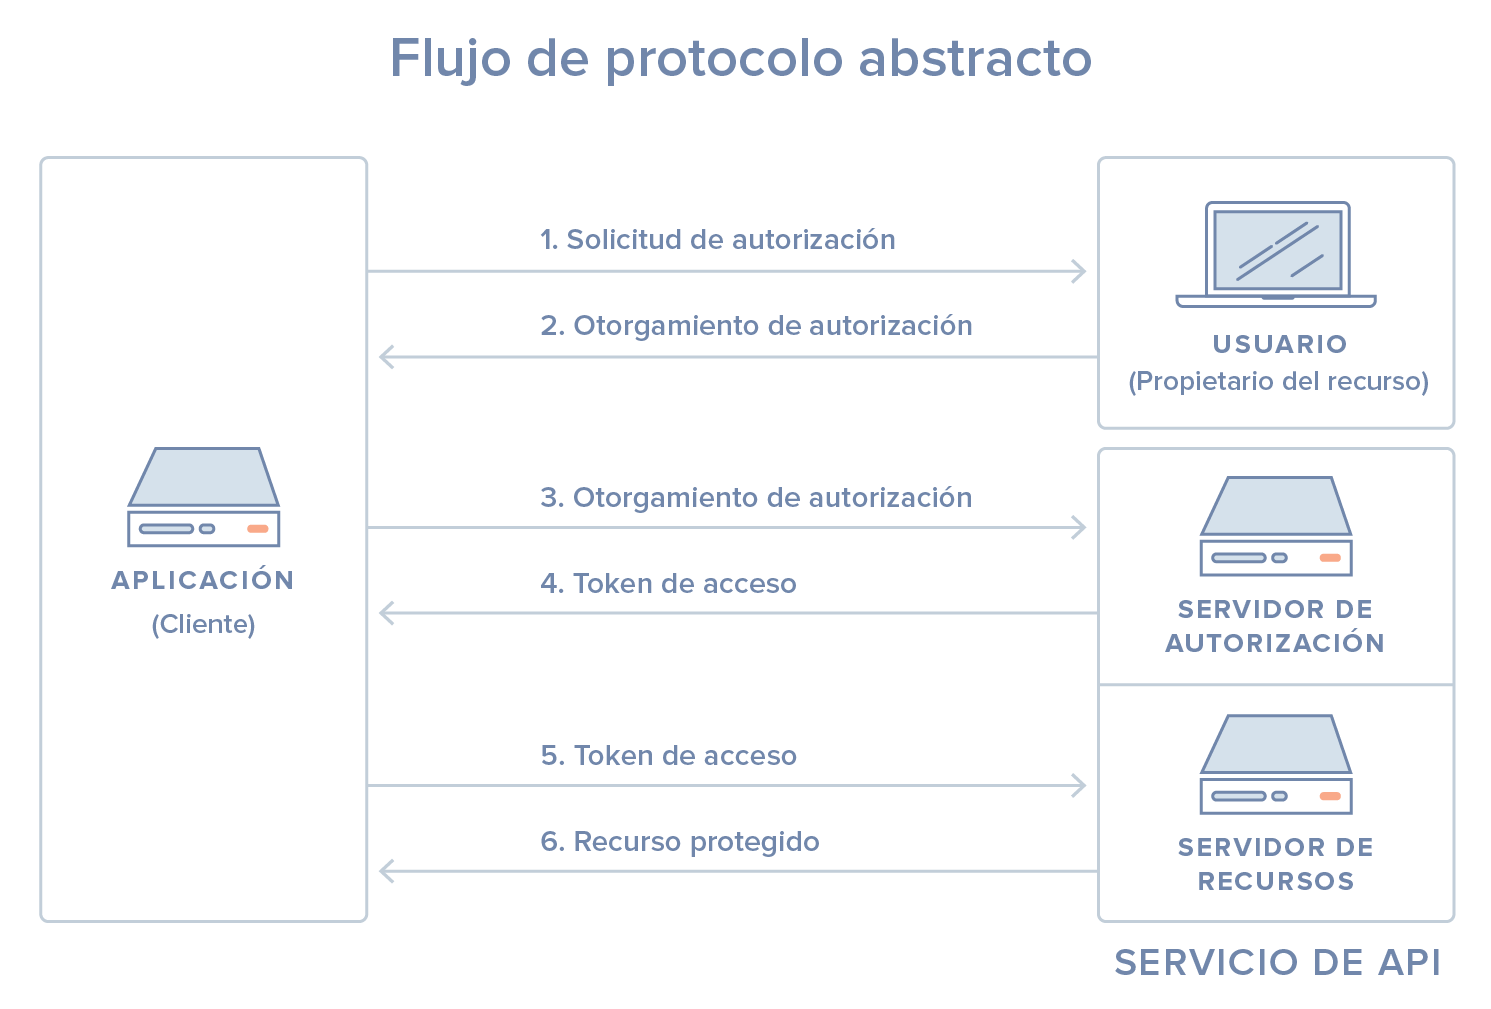
\includegraphics[scale=0.50]{TT/img/analisis/Abstract-Protocol-Flow-Spanish@2x.png}
    \caption{Flujo de protocolo abstracto. \cite{Anicas2018}}
    \label{graphic:OAuth2}
\end{figure}

A continuación se realiza una explicación mas detallada de los pasos del diagrama \ref{graphic:OAuth2}:

\begin{enumerate}
    \item La aplicación solicita autorización para acceder a los recursos de servicio del usuario.
    \item Si el usuario autoriza la solicitud, la aplicación recibe la autorización.
    \item La aplicación solicita al servidor de autorización (API), presentando la autenticación de su identidad y la autorización otorgada La aplicación solicita al servidor de autorización (API) un token de acceso presentando la autenticación de su propia identidad y la autorización otorgada.
    \item Si la identidad de la aplicación es autenticada y la autorización es válida, el servidor de autorización (API) emite un token de acceso a la aplicación. La autorización finaliza.
    \item La aplicación solicita el recurso al servidor de recursos (API) y presenta el token de acceso para autenticarse.
    \item Si el token de acceso es válido, el servidor de recursos (API) provee el recurso a la aplicación.
\end{enumerate}

El flujo de este proceso será diferente dependiendo del tipo de autorización que se escoja, sin embargo, esta es la idea general. \cite{Anicas2018}

\subsection{Tipos de clientes}

\begin{itemize}
    \item \textbf{Clientes confidenciales: }son aquellos que son capaces de guardar una contraseña sin que sea expuesta. Una aplicación compilada es un ejemplo.
    \item \textbf{Clientes públicos: }son aquellos que no son capaces de mantener esta contraseña a salvo, un buen ejemplo son las aplicaciones web.
\end{itemize}

\subsection{Tipos de concesión (Gran types)}
Con esta estructura disponemos de diferentes tipos de concesión, a continuación se muestran algunas de las más conocidas:
\begin{itemize}
    \item \textbf{Código de autorización: }usado con aplicaciones del lado del servidor.
    \item \textbf{Implícito: }utilizado con aplicaciones móviles o aplicaciones web (aplicaciones que se ejecutan en el dispositivo del usuario)
    \item \textbf{Credenciales de contraseña del propietario del recurso: }utilizado con aplicaciones confiables, como aquellas pertenecientes al servicio.
    \item \textbf{Credenciales del cliente: }basada en las credenciales de cliente.
\end{itemize}

Para el desarrollo de este proyecto se usará el tipo de otorgamiento: Credenciales de contraseña del propietario del recurso, este mismo se describirá a continuación.

\subsection{Tipo de otorgamiento: Credenciales de contraseña del propietario del recurso}
Con el tipo de otorgamiento de credenciales de contraseña del propietario del recurso, el usuario proporciona sus credenciales de servicio (nombre de usuario y contraseña) directamente a la aplicación, la cual utiliza dichas credenciales para obtener del servicio un token de acceso. \cite{Anicas2018}

\subsubsection{Flujo de credenciales de contraseña}
Después de que el usuario proporcione sus credenciales a la aplicación, ésta solicitará un token de acceso desde el servidor de autorizaciones. La solicitud POST puede ser similar a lo siguiente:

\textit{https://oauth.example.com/token?grant-type=password \&username=USERNAME\& password= PASSWORD \&client-id=CLIENT-ID}

Si se comprueban las credenciales del usuario, el servidor de autorización devuelve un token de acceso a la aplicación.\cite{Anicas2018}

%
\section{Justificación de las herramientas elegidas}
Las herramientas, protocolos, el lenguaje y frameworks descritos anteriormente fueron elegidos para desarrollar la solución propuesta. 

Python es el lenguaje de programación que su facilidad de uso y aprendizaje junto con su continua optimización es la elección ideal para este proyecto, sus continuas correcciones y actualizaciones da fiabilidad a los proyectos realizados.

FastAPI es desarrollado con Python, por lo cual, aprovecha los beneficios de este y facilita aún mas el crear una API desde cero ya que es una herramienta usada en la industria lo que da certeza de su fiabilidad y por lo tanto, tiene madurez para que el desarrollo del proyecto sea estable, lo que genera una buena comunidad de desarrollo que se aprovecha para aclarar dudas y resolver errores, todo esto es posible con su buena documentación y continua actualización de esta misma. Su creador ha generado ejemplos para familiarizarse con la herramienta y es documentada para su fácil comprensión, lo cual fue aprovechado para crear este proyecto.  Con FastAPI se resuelve la característica planteada que es el crear un sistema en la web que permita realizar los cálculos y peticiones necesarias para realizar las predicciones, que es el propósito de este proyecto.

Oauth 2 es una herramienta/protocolo que añade seguridad al proyecto \cite{Anicas2018, Magana2020}, que permite blindar los puntos de acceso de la API de usos no autorizados, esto es implementado para permitir el acceso al servidor de recursos y hacer uso de estos siempre y cuando, se tenga una cuenta válida y activa en el sistema.

\section{Metodología}
Para este trabajo terminal se utilizará la metodología de \acrfull{RAD}, dado que el tiempo de desarrollo es corto, esta metodología permite centrarse en el producto final, hace hincapié en el desarrollo de prioridades y la definición de los plazos de entrega, si estos empiezan a atrasarse permite la reducción de requisitos para el ajuste y de esta manera no prolongar la fecha limite de entrega. Por otro lado la participación de los usuarios es necesaria para el diseño del sistema.\cite{dra}

\begin{figure}[!ht]
    \centering
    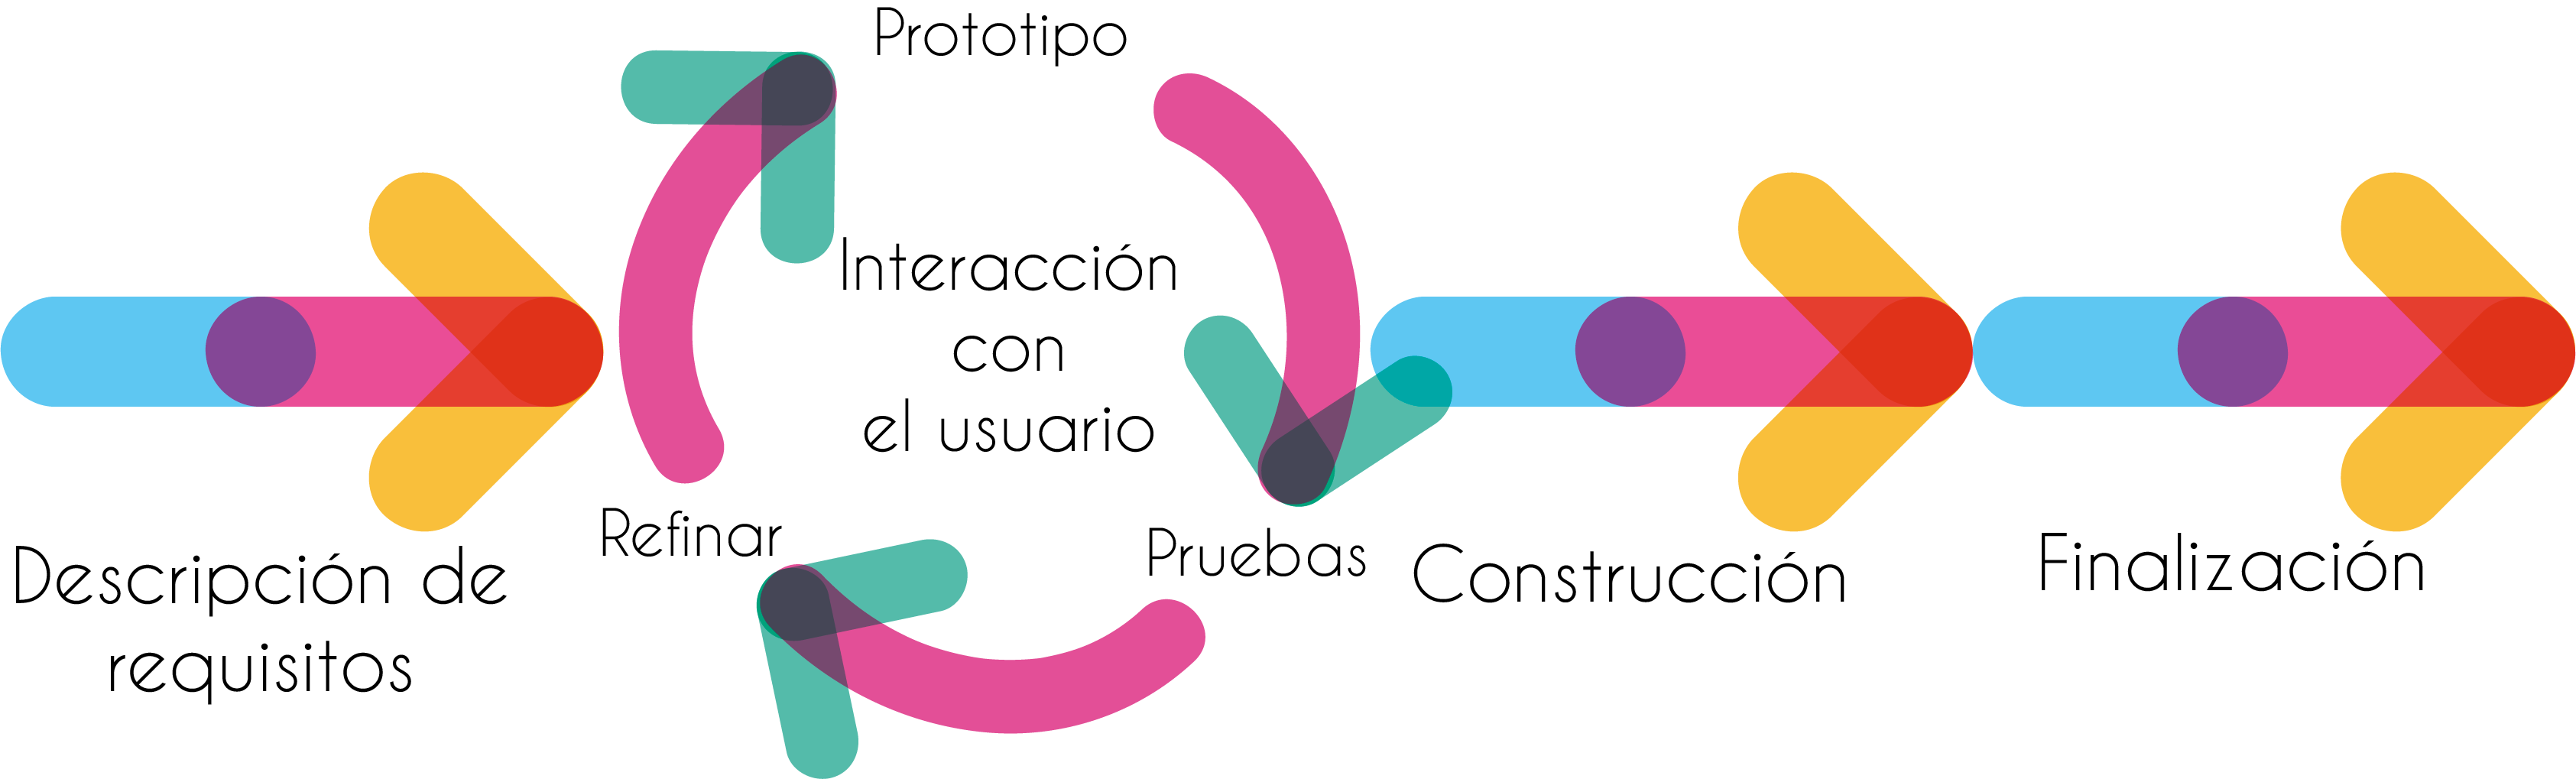
\includegraphics[scale=0.50]{TT/img/metodología/RAD.png}
    \caption{Desarrollo rápido de aplicaciones}
    \label{graphic:RAD}
\end{figure}

\section{Requerimientos}
Hasta este punto, se ha presentado conceptos teóricos con los que el sistema se basará para su desarrollo y se ha realizado un análisis de las herramientas y técnicas de programación que se usarán a lo largo del desarrollo del sistema, a continuación se describirá toda la funcionalidad que este tendrá.

\subsection{Requerimientos funcionales}
Para la comprensión de las tablas que describen los requerimientos son \textbf{RFSXXX} siendo su significado \textit{Requerimiento funcional de Software} y el último es \textbf{RNSXXX} siendo su significado \textit{Requerimiento no funcional de Software}.

\begin{longtable}{|c|m{4cm}|m{9.5cm}|}
    \hline
    \rowcolor[HTML]{3531FF} 
    {\color[HTML]{FFFFFF} Id} &{\color[HTML]{FFFFFF}Nombre} & {\color[HTML]{FFFFFF} Descripción} \\ \hline
    \endfirsthead
    \hline
    \rowcolor[HTML]{3531FF} 
    {\color[HTML]{FFFFFF} Id} &{\color[HTML]{FFFFFF}Nombre} & {\color[HTML]{FFFFFF} Descripción} \\
    \hline 
    \endhead
    % aquí añadimos el fondo de todas las hojas, excepto de la última.
    \multicolumn{3}{c}{Sigue en la página siguiente.}
    \endfoot
    % aquí añadimos el fondo de la última hoja.
    \endlastfoot
    RFS001&Analizar partido político&Poder analizar únicamente un partido político.\\ \hline
    RFS002&Analizar un conjunto de partidos políticos&Poder analizar un conjunto de partidos políticos que se encuentran en competencia. \\ \hline
    RFS003&Usuarios&El sistema debe permitir el registro de usuarios. \\ \hline
    RFS004&Encuestas&Permitir la creación de encuestas mediante el uso de usuarios registrados. \\ \hline
    RFS005&Visualización de datos&Permitir la visualización de los resultados obtenidos de encuestas a todos los usuarios del sistema. \\ \hline
    RFS006&Guardar encuestas&El sistema debe guardar las encuestas creadas por los usuarios. \\\hline
    RFS007&Encuestas&Las encuestas solo podrán ser de opción múltiple. \\ \hline
    RFS008&Asignación de peso para respuestas&El sistema debe de poder dejar al usuario registrado asignar y editar pesos a las respuestas disponibles de cada pregunta. \\ \hline
    RFS009&CRUD preguntas&El sistema debe dejar al usuario crear, editar, eliminar y guardar las preguntas de la encuesta. \\ \hline
    RFS010&Resultado de encuesta&El sistema debe mostrar los resultados al finalizar la encuesta con el porcentaje de éxito o fracaso.\\ \hline
    \caption{Requerimientos funcionales de la aplicación}
    \label{table:RFS}
\end{longtable}
\subsection{Requerimientos no funcionales}
Por otro lado, es necesario saber cuales son los requerimientos no funcionales, teniendo ambos tipos de requerimientos, nos damos una idea mas clara sobre que desarrollar y como hacerlo.

\begin{longtable}{|c|m{4cm}|m{9.5cm}|}
    \hline
    \rowcolor[HTML]{3531FF} 
    {\color[HTML]{FFFFFF} Id} &{\color[HTML]{FFFFFF}Nombre} & {\color[HTML]{FFFFFF} Descripción} \\ \hline
    \endfirsthead
    \hline
    \rowcolor[HTML]{3531FF} 
    {\color[HTML]{FFFFFF} Id} &{\color[HTML]{FFFFFF}Nombre} & {\color[HTML]{FFFFFF} Descripción} \\
    \hline 
    \endhead
    % aquí añadimos el fondo de todas las hojas, excepto de la última.
    \multicolumn{3}{c}{Sigue en la página siguiente.}
    \endfoot
    % aquí añadimos el fondo de la última hoja.
    \endlastfoot
    RNS001&Factor de error&El factor de error que podría tener el sistema sería hasta de 30\%* aproximadamente.\\ \hline
    RNS002&Rango de pesos&El rango en los pesos de las respuestas debe ser de 1 a 5.\\ \hline
    \caption{Requerimientos no funcionales de la aplicación}
    \label{table:RNS}
\end{longtable}

\textit{* El porcentaje de error es propuesto con base en la publicación de Galam 'The dynamics of minority opinions in democratic debate', donde propone un porcentaje de 30\% para que el cambio de opinión en una determinada población cambie a través del tiempo. \cite{Galam2004}}

\textit{En la literatura consultada (\cite{Galam.1986, Galam2000, Galam2004, Galam1998, Galam2001}) refiere que el 30\% es un margen de error valido en este campo de estudio, dado que existen variables como la variación de la población inicial de un proceso electoral al siguiente, situaciones como abstención, voto nulo o voto foráneo no se pueden considerar y no pueden ser descritas matemáticamente e influyen en el comportamiento de una población.\cite{MarioH.RamirezDiaz2014}}
